\subsection{Experimental Setup}
\label{subsec:setup}

\subsubsection{Layered benchmark protocol}

The empirical study is organized in three layers because the paper addresses three questions. The first question is \emph{whether the proposed pipeline can reliably convert a strong fractional trajectory into a strictly feasible mixed-integer incumbent}. For that purpose we retain the four-instance audited benchmark used throughout Plan~1: p0033, p0201, p0282, and knapsack\_50. These instances are small enough that every candidate solution can be inspected carefully, yet still diverse enough to expose the core feasibility transition studied in the paper.

The second question is \emph{whether the same architecture remains competitive once we move from illustrative audited cases to a standardized MIPLIB 2017 benchmark protocol}. To answer that question, we parsed the official MIPLIB 2017 benchmark-v2 test set and the official v36 \texttt{.solu} reference file, then filtered instances by predeclared structural rules rather than by ex post performance: known official reference value, 100--3000 variables, 50--2500 constraints, at least 20 integer variables, integer ratio at least 0.30, and at most 60{,}000 nonzeros. These rules yielded a 29-instance candidate pool. From that pool we selected twelve size-diverse instances by a deterministic stratified procedure and copied only those files into the local \texttt{Plan 1/data/miplib2017\_sec} directory. The resulting official subset spans 274--2500 variables and 233--2107 constraints, with a median integer ratio above 0.93; instance-level names and sizes are reported in Table~\ref{tab:extended_benchmark}.

Finally, to position the method against widely used intelligent population heuristics, we extracted the six smallest instances from the official subset and ran an additional representative comparison against GA, DE, SHADE, and SL-PSO, together with the archived implementation variants Standard Pop-PDHG and Quantum Pop-PDHG. This third layer is not used to replace the fully audited four-instance feasibility benchmark; rather, it tests whether the proposed hybrid feasibility-recovery architecture occupies a competitive position relative to established population-based baselines when all methods are evaluated under the same repaired feasibility audit. To keep the data chain auditable, the raw result files retain the archived implementation labels, while the manuscript refers to them conceptually as the baseline and hybrid variants.

\subsubsection{Baselines, repeated runs, and audited metrics}

Our primary controlled comparator remains \emph{Standard Pop-PDHG}, obtained by disabling the barrier-crossing and progressive integrality-projection enhancements while preserving the common population backbone, PDHG updates, and repair infrastructure. Throughout the narrative below, we refer to the proposed method as HP-PDHG; in the stored implementation and result tables, the same solver appears under the legacy name \emph{Quantum Pop-PDHG}. Gurobi~13.0.1 \cite{gurobi2024} provides the exact-solver reference. For the official MIPLIB 2017 extension we use the official v36 \texttt{.solu} file as the authoritative objective reference, while a 60-second Gurobi run is retained as an additional local sanity check.

For the population-based comparison we evaluate four broader metaheuristics: a real-coded genetic algorithm, DE, SHADE, and SL-PSO \cite{storn1997de,tanabe2013shade,cheng2015slpso}. To make the comparison fair, these baselines are not judged on raw penalized fitness alone. Instead, after each run we pass the incumbent through the same audited feasibility-repair layer used by the proposed method, then re-evaluate it against the \emph{original} constraint senses, bound constraints, and integrality conditions. This common post-processing step is important because otherwise different solvers would be compared through incompatible definitions of constraint satisfaction.

Every reported value in the paper therefore corresponds to one of three audited quantities: objective value, maximum primal violation with respect to the original MPS model, and feasibility status after explicit rechecking of integrality and bounds. For the four-instance audited benchmark we also report absolute percentage gap to the exact Gurobi optimum, and we additionally rerun that benchmark over 20 seeds to quantify robustness. For the official benchmark extension and the population-based baseline study, the main performance variable is the final maximum violation, because many runs remain infeasible under the fixed budget and any ``objective'' attached to an infeasible point is only diagnostic. The official extension uses five random seeds per solver, and the representative population-based baseline study uses the same five-seed protocol.

\subsubsection{Implementation, hardware, and reproducibility}

All experiments were executed on a MacBook Pro with Apple M4 Pro CPU (12 cores) and 24\,GB unified memory using Python~3.13, NumPy, SciPy, and Gurobi. The key correction relative to earlier project iterations is that the final experimental chain no longer relies on permissive feasibility checks. Earlier legacy scripts occasionally hard-coded optimal values, ignored original constraint senses, or failed to recompute the objective after repair. The audited Plan~1 pipeline corrects those issues. In particular, the final benchmark scripts use the original MPS files, the official \texttt{.solu} references for MIPLIB 2017, original bound data, and explicit post-repair verification. For a paper whose central claim is feasibility recovery rather than relaxed objective quality, that audit is not a cosmetic detail; it is part of the contribution.

\subsection{Audited Feasibility-Recovery Benchmark}
\label{subsec:main_results}

Table~\ref{tab:main_results} reports the main audited benchmark. The pattern is unambiguous. The baseline Pop-PDHG variant drives the relaxation to attractive objective regions on all four instances, but it remains infeasible after explicit rechecking. By contrast, HP-PDHG recovers strict feasibility on all four. It matches the Gurobi optimum on p0033, reaches a feasible incumbent within 2.21\% of optimum on p0201, crosses the p0282 near-feasibility barrier with only a 0.16\% gap, and returns a feasible solution within 0.54\% of optimum on knapsack\_50.

\begin{table}[htbp]
\centering
\caption{Audited four-instance feasibility-recovery benchmark. Gaps are absolute percentages relative to the Gurobi optimum. For infeasible solvers, the objective is diagnostic only and does not constitute a valid primal bound, which is why feasibility status remains the primary operational criterion.}
\label{tab:main_results}
\small
\resizebox{\textwidth}{!}{%
\begin{tabular}{llccccc}
\toprule
\textbf{Instance} & \textbf{Solver} & \textbf{Objective} & \textbf{Abs.\ gap (\%)} & \textbf{Max violation} & \textbf{Time (s)} & \textbf{Feasible} \\
\midrule
\multirow{3}{*}{p0033}
& Gurobi & -68.0000 & -- & 0 & 0.004 & Yes \\
& Baseline Pop-PDHG & -86.0000 & 26.47 & 1.4409 & 0.369 & No \\
& \textbf{HP-PDHG} & \textbf{-68.0000} & \textbf{0.00} & \textbf{0} & \textbf{0.473} & \textbf{Yes} \\
\midrule
\multirow{3}{*}{p0201}
& Gurobi & -226.0000 & -- & 0 & 0.007 & Yes \\
& Baseline Pop-PDHG & -239.0000 & 5.75 & 1.8988 & 2.080 & No \\
& \textbf{HP-PDHG} & \textbf{-221.0000} & \textbf{2.21} & \textbf{0} & \textbf{2.707} & \textbf{Yes} \\
\midrule
\multirow{3}{*}{p0282}
& Gurobi & -7899.4132 & -- & 0 & 0.013 & Yes \\
& Baseline Pop-PDHG & -7888.3187 & 0.14 & 0.0805 & 2.956 & No \\
& \textbf{HP-PDHG} & \textbf{-7887.0719} & \textbf{0.16} & \textbf{$9.87\times10^{-7}$} & \textbf{4.234} & \textbf{Yes} \\
\midrule
\multirow{3}{*}{knapsack\_50}
& Gurobi & -2051.0000 & -- & 0 & 0.001 & Yes \\
& Baseline Pop-PDHG & -2076.0000 & 1.22 & 3.4000 & 0.526 & No \\
& \textbf{HP-PDHG} & \textbf{-2040.0000} & \textbf{0.54} & \textbf{0} & \textbf{0.640} & \textbf{Yes} \\
\bottomrule
\end{tabular}%
}
\end{table}

Two details are worth emphasizing. First, the objective values of the infeasible baseline Pop-PDHG rows are often numerically attractive, but they are scientifically secondary because they do not correspond to valid incumbents. The p0282 case is especially instructive: the baseline variant appears superficially competitive on objective value, yet it still violates the original model by $8.05\times 10^{-2}$. HP-PDHG sacrifices only a small additional amount of objective quality in exchange for verified feasibility. Second, the p0033 row shows that the proposed pipeline is not merely a ``repair to any feasible point'' strategy. When the instance geometry is favorable, the method can recover feasibility without paying an objective premium at all.

The same message survives aggressive repetition. We reran the four audited instances over 20 seeds per solver, yielding 80 paired runs. HP-PDHG produced a verified feasible incumbent in all 80 runs, whereas the baseline Pop-PDHG variant produced none. The exact paired sign test on discordant feasibility outcomes gives $p=8.27\times10^{-25}$, and the paired Wilcoxon test on audited primal violations gives $p=2.75\times10^{-15}$. These repeated-run results matter because they convert Table~\ref{tab:main_results} from a visually compelling but small benchmark into a statistically overwhelming robustness result for the specific feasibility-recovery claim made in the paper.

Figure~\ref{fig:p0282_tradeoff} visualizes the p0282 mechanism from another angle. The baseline variant sits in a low-objective but still infeasible basin. The hybrid variant moves slightly away from that basin in objective space but crosses the final feasibility barrier. In other words, the contribution of the method is not better local optimization on the relaxation; it is a more reliable transition from a strong fractional point to an admissible integer point.

\begin{figure}[htbp]
\centering
\begin{subfigure}[b]{0.31\textwidth}
    \centering
    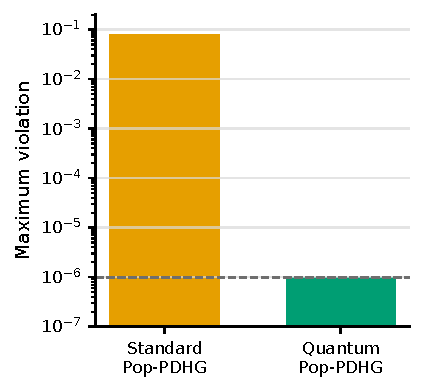
\includegraphics[width=\textwidth]{figures/p0282_feasibility_nature.pdf}
    \caption{Maximum violation}
\end{subfigure}
\hfill
\begin{subfigure}[b]{0.31\textwidth}
    \centering
    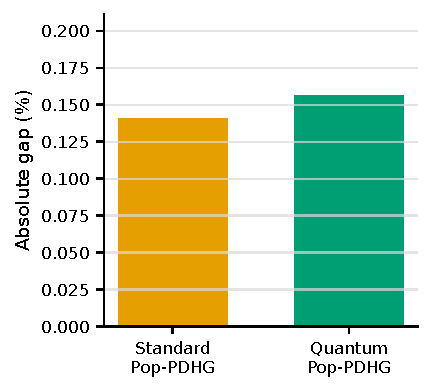
\includegraphics[width=\textwidth]{figures/p0282_gap_nature.pdf}
    \caption{Absolute objective gap}
\end{subfigure}
\hfill
\begin{subfigure}[b]{0.31\textwidth}
    \centering
    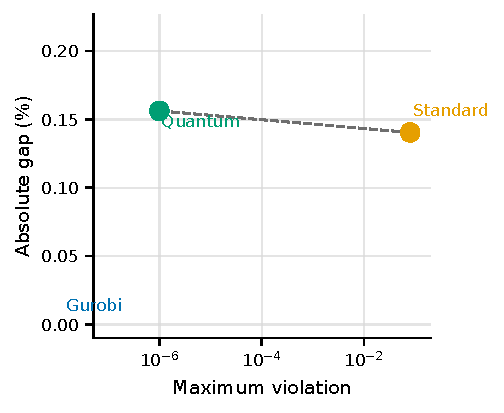
\includegraphics[width=\textwidth]{figures/p0282_tradeoff_nature.pdf}
    \caption{Feasibility--gap trade-off}
\end{subfigure}
\caption{Audited behavior on p0282. The baseline variant reaches a strong but invalid near-feasible point, whereas HP-PDHG crosses the final feasibility barrier with only a modest additional objective sacrifice, illustrating the practical value of converting a good fractional plan into an admissible decision.}
\label{fig:p0282_tradeoff}
\end{figure}

\subsection{Official MIPLIB 2017 Extension}
\label{subsec:extended_official}

The four-instance audited benchmark establishes that the method can perform the central feasibility transition. The next question is whether the same behavior persists on a standardized official benchmark subset selected without looking at solver outcomes. Table~\ref{tab:extended_benchmark} addresses that question on the twelve-instance MIPLIB 2017 extension.

\begin{table}[htbp]
\centering
\caption{Official MIPLIB 2017 extension under a fixed budget of 1000 iterations and five random seeds. Reported violations are per-instance means after audited repair and rechecking, so the table measures how effectively each method reduces residual infeasibility when full closure is still difficult.}
\label{tab:extended_benchmark}
\small
\resizebox{\textwidth}{!}{%
\begin{tabular}{lcccccc}
\toprule
\textbf{Instance} & \textbf{$n$} & \textbf{$m$} & \textbf{Integer ratio} & \textbf{Baseline mean violation} & \textbf{HP-PDHG mean violation} & \textbf{Reduction (\%)} \\
\midrule
glass4 & 322 & 396 & 0.94 & $3.00\times10^{5}$ & $3.00\times10^{5}$ & 0.0 \\
neos-3046615-murg & 274 & 498 & 0.93 & 53.60 & 20.00 & 62.7 \\
neos-2657525-crna & 524 & 342 & 1.00 & $5.71\times10^{3}$ & $2.65\times10^{3}$ & 53.6 \\
ic97\_potential & 728 & 1046 & 0.72 & 33.92 & 34.94 & -3.0 \\
cod105 & 1024 & 1024 & 1.00 & 0.00 & 0.00 & 0.0 \\
gmu-35-40 & 1205 & 424 & 1.00 & 19.52 & 13.54 & 30.6 \\
neos-4954672-berkel & 1533 & 1848 & 0.41 & $7.29\times10^{3}$ & $7.21\times10^{3}$ & 1.0 \\
mcsched & 1747 & 2107 & 1.00 & 934.80 & 1069.48 & -14.4 \\
gmu-35-50 & 1919 & 435 & 1.00 & 14.36 & 10.30 & 28.3 \\
50v-10 & 2013 & 233 & 0.82 & 148.14 & 136.11 & 8.1 \\
p200x1188c & 2376 & 1388 & 0.50 & $2.58\times10^{3}$ & $4.71\times10^{2}$ & 81.8 \\
beasleyC3 & 2500 & 1750 & 0.50 & 21.72 & 15.82 & 27.2 \\
\bottomrule
\end{tabular}%
}
\end{table}

Several points emerge from this table. First, the official extension is markedly harder than the audited four-instance benchmark. Even with 1000 iterations and five seeds, the only instance solved to strict feasibility by both methods in all runs is cod105. This is useful information rather than a failure of reporting. It shows that once the benchmark is broadened, the scientific question shifts from ``can the method ever cross the feasibility barrier?'' to ``does the proposed mechanism reduce the residual distance to feasibility more effectively than the baseline under a fixed computation budget?'' That is precisely why the maximum violation becomes the primary metric in the extension.

Second, the added hybrid mechanisms now produce a broader and statistically stronger directional advantage on the official subset. HP-PDHG lowers the mean audited violation on eight of the twelve instances, ties on two, and loses on two; the median per-instance change is a 27.2\% reduction. The strongest improvements occur on p200x1188c (81.8\%), neos-3046615-murg (62.7\%), neos-2657525-crna (53.6\%), gmu-35-40 (30.6\%), gmu-35-50 (28.3\%), and beasleyC3 (27.2\%). The mixed cases remain informative: ic97\_potential is a near-tie with a slight disadvantage for HP-PDHG, and mcsched remains a genuine counterexample.

Third, the extension provides a more favorable but still honest calibration of the method's current maturity. The paired Wilcoxon test on per-instance mean violations now favors HP-PDHG at the 5\% level ($p=0.032$). We therefore have stronger evidence than before that the proposed architecture reduces distance to feasibility on official instances under a fixed budget. At the same time, the interpretation should remain disciplined: two instances are exact ties, glass4 is a pathological outlier, and the strict-feasibility count does not yet show broad large-scale closure beyond cod105. The contribution supported by these data is therefore \emph{improved official-benchmark feasibility reduction}, not universal official-benchmark dominance.

These trends are summarized visually in Figure~\ref{fig:sec_official}. The figure should be read as an extension study, not as the central proof of feasibility recovery.

\begin{figure}[htbp]
\centering
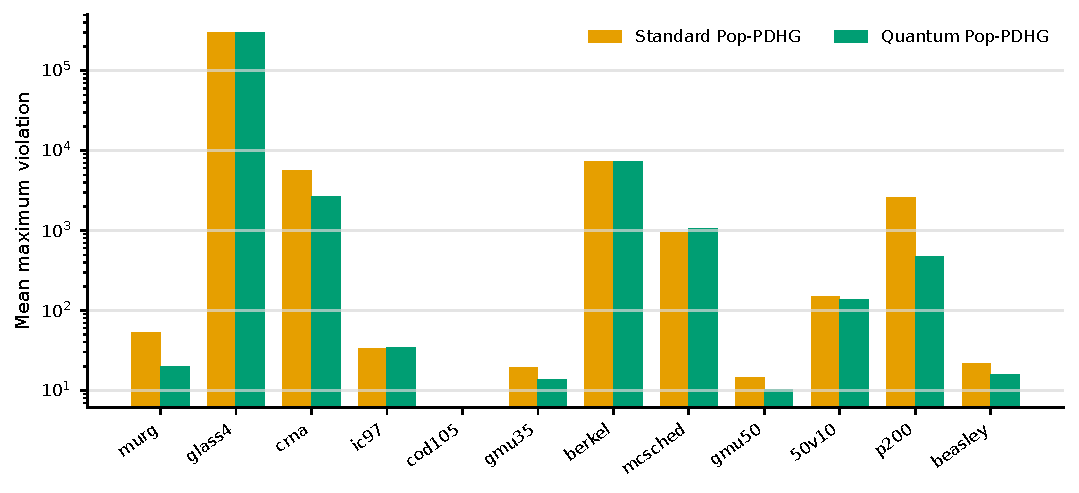
\includegraphics[width=0.92\textwidth]{figures/sec_official_benchmark_nature.pdf}
\caption{Official MIPLIB 2017 extension. Bars report mean audited maximum violation over five seeds. HP-PDHG improves eight instances, ties two, and loses two under a fixed 1000-iteration budget, which supports the view that the method is most useful as a feasibility-reduction module on harder instances.}
\label{fig:sec_official}
\end{figure}

\subsection{Comparison with Population-Based Metaheuristics}
\label{subsec:sec_baselines}

The population-based baseline study asks a different but complementary question: if we ignore exact proof of optimality and compare only population-based heuristics under the same repaired feasibility audit, where does HP-PDHG sit relative to standard intelligent search methods? Table~\ref{tab:sec_rank_table} summarizes the answer on the six smallest official instances from the 12-instance official subset, using per-instance mean audited violation and Friedman ranks.

\begin{table}[htbp]
\centering
\caption{Average Friedman ranks on the six-instance representative population-based baseline study. Lower is better. The table is intended to show comparative placement among intelligent heuristics rather than universal pairwise dominance.}
\label{tab:sec_rank_table}
\small
\begin{tabular}{lcc}
\toprule
\textbf{Solver} & \textbf{Average rank} & \textbf{Mean violation} \\
\midrule
HP-PDHG & \textbf{1.75} & $5.05\times10^{4}$ \\
SHADE & 2.67 & $1.09\times10^{6}$ \\
Baseline Pop-PDHG & 3.08 & $5.10\times10^{4}$ \\
SL-PSO & 4.00 & $1.99\times10^{5}$ \\
DE & 4.67 & $6.55\times10^{6}$ \\
GA & 4.83 & $1.59\times10^{6}$ \\
\bottomrule
\end{tabular}
\end{table}

The first observation is encouraging for the proposed method: HP-PDHG attains the best average rank (1.75), ahead of SHADE, the baseline Pop-PDHG variant, SL-PSO, DE, and GA. The second observation is equally important: this leadership is not uniform across all instances. On neos-3046615-murg and gmu-35-40, HP-PDHG is clearly strongest. On glass4 and cod105, the two PDHG variants are tied at the best observed violation. On neos-2657525-crna, HP-PDHG is near-best but SHADE performs slightly better. On ic97\_potential, the baseline variant is marginally better than the hybrid one. This is exactly the kind of pattern a credible hybrid heuristic should produce: strong average placement and identifiable strengths, but not artificial claims of instance-by-instance invincibility.

This mixture of wins, ties, and close second-place finishes is visible in Figures~\ref{fig:sec_ranks} and~\ref{fig:sec_heatmap}. The rank plot captures the overall pattern across instances; the heatmap shows that the proposed method is not simply globally dominant, but rather occupies a competitive niche. It tends to be strongest when relaxation information remains useful and the feasibility transition is the real bottleneck. From a scientific perspective, this is exactly the kind of evidence a hybrid heuristic should provide: not the fantasy of universal dominance, but a clear statement of where the method fits among established intelligent baselines.

The nonparametric tests tell the same story in a more disciplined way. The overall Friedman test is now significant at the 5\% level ($p=0.016$), which supports the claim that the six solvers are not statistically indistinguishable on this representative subset. However, the Holm-adjusted pairwise Wilcoxon tests remain conservative, so the correct interpretation is \emph{significant overall ordering with cautious post-hoc claims}, not pairwise universal superiority. Within that boundary, HP-PDHG still emerges as the best-ranked method on average.

\begin{figure}[htbp]
\centering
\begin{subfigure}[b]{0.43\textwidth}
    \centering
    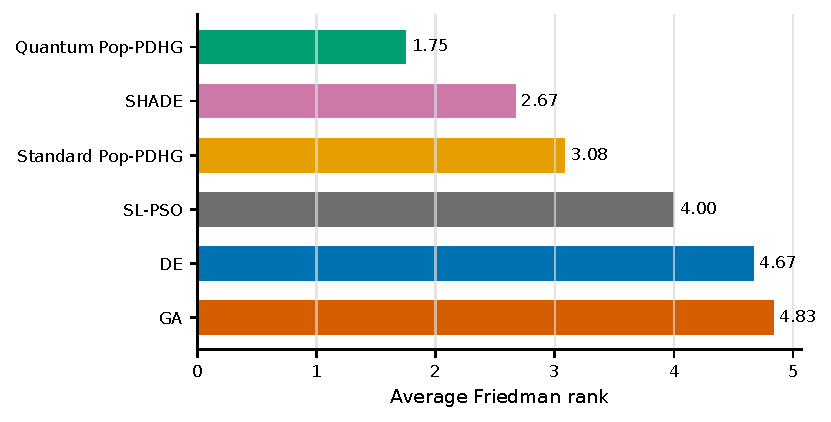
\includegraphics[width=\textwidth]{figures/sec_metaheuristic_ranks_nature.pdf}
    \caption{Average ranks}
    \label{fig:sec_ranks}
\end{subfigure}
\hfill
\begin{subfigure}[b]{0.53\textwidth}
    \centering
    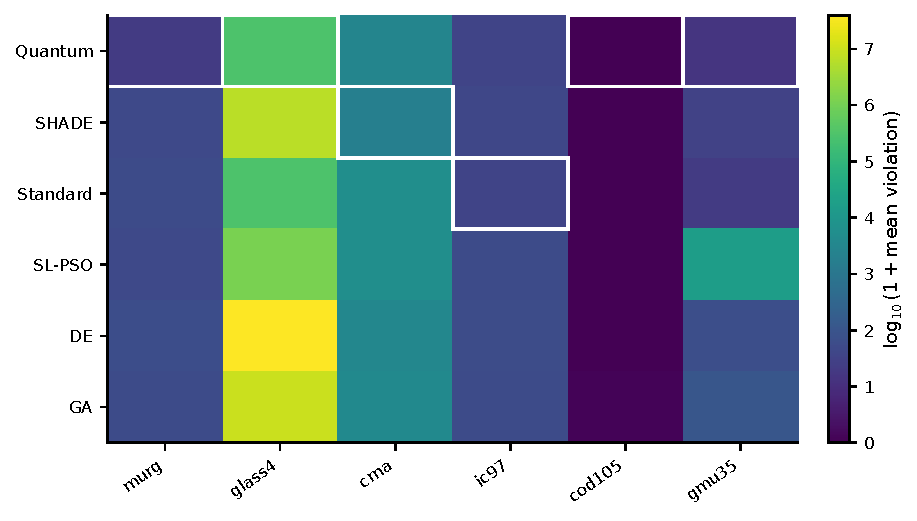
\includegraphics[width=\textwidth]{figures/sec_metaheuristic_heatmap_nature.pdf}
    \caption{Per-instance violation heatmap}
    \label{fig:sec_heatmap}
\end{subfigure}
\caption{Representative comparison against population-based intelligent baselines. The archived solver variant labeled Quantum Pop-PDHG, corresponding to HP-PDHG in the manuscript, attains the best average rank, while the heatmap clarifies that its advantage is instance dependent rather than universal. White outlines indicate the best solver on each instance and highlight the heterogeneity that motivates hybrid or portfolio use.}
\label{fig:sec_meta}
\end{figure}

\subsection{Ablation of the Added Mechanisms}
\label{subsec:ablation}

The current implementation includes several modules that were added during the later development stages of Plan~1, including the second-stage feasibility-first controller, the projection-based repair path, and the progressive integrality-projection schedule. The ablation study isolates the most practically important components. Table~\ref{tab:ablation} aggregates the corrected ablation results across the four-instance audited benchmark.

\begin{table}[htbp]
\centering
\caption{Aggregated ablation results on the four-instance audited benchmark. ``Feasible instances'' counts how many of the four instances end in verified strict feasibility. Mean feasible gap is reported only over successful runs, allowing the contribution of each module to be interpreted separately.}
\label{tab:ablation}
\small
\resizebox{\textwidth}{!}{%
\begin{tabular}{lcccc}
\toprule
\textbf{Configuration} & \textbf{Feasible instances} & \textbf{Mean feasible gap (\%)} & \textbf{Mean runtime (s)} & \textbf{Mean tunnel success rate (\%)} \\
\midrule
Base Pop-PDHG & 0/4 & -- & 1.98 & 0.0 \\
+ Barrier-Aware Perturbation & 0/4 & -- & 1.98 & 28.5 \\
+ Progressive Projection & 4/4 & 0.727 & 2.51 & 0.0 \\
+ HMC Dynamics & 0/4 & -- & 1.98 & 0.0 \\
Full HP-PDHG & 4/4 & 0.726 & 2.51 & 42.6 \\
\bottomrule
\end{tabular}
}
\end{table}

The qualitative message of Table~\ref{tab:ablation} is stronger than any single row. The barrier-aware perturbation alone changes exploration statistics and produces accepted non-local moves, but it does not by itself recover strict feasibility. HMC dynamics, in the present implementation, also do not change that conclusion. Progressive projection is the turning point: once staged integrality enforcement is turned on, the solver crosses from attractive but infeasible trajectories to verified feasible incumbents on all four audited cases. The full method then preserves that feasibility profile while increasing the accepted-jump rate, which supports the interpretation that the non-local perturbation is \emph{complementary} rather than \emph{sufficient}. It helps diversify search, but the actual feasibility transition is carried primarily by projection and repair.

\subsection{Parameter Sensitivity}
\label{subsec:sensitivity}

We additionally reran the parameter-sensitivity study on the corrected code path, for a total of 390 audited runs. The purpose of this study is not exhaustive hyperparameter tuning; it is to determine whether the proposed method depends on a narrow and fragile set of parameter values. The answer is encouraging. Across the easy audited instances, the method operates on a broad stable plateau rather than a knife-edge optimum.

Figure~\ref{fig:sensitivity} summarizes two representative trends. Increasing the tunnel interval from 25 toward 100--200 typically improves the quality of accepted jumps because the population has more time to reshape the relaxation trajectory between non-local transitions. At the same time, larger populations increase runtime roughly monotonically, but they do not produce a corresponding monotonic gain in final solution quality on the easy audited instances. This is exactly the sensitivity pattern one would hope for in a practical heuristic: the parameters matter, but the mainline configuration is not rescued by a single exceptional setting.

\begin{figure}[htbp]
\centering
\begin{subfigure}[b]{0.46\textwidth}
    \centering
    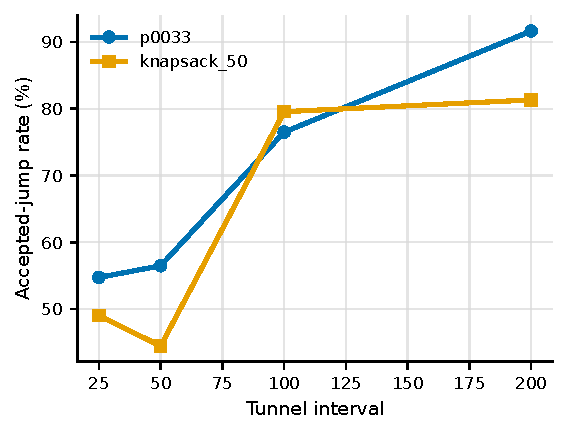
\includegraphics[width=\textwidth]{figures/sensitivity_tunnel_interval_nature.pdf}
    \caption{Tunnel interval}
\end{subfigure}
\hfill
\begin{subfigure}[b]{0.46\textwidth}
    \centering
    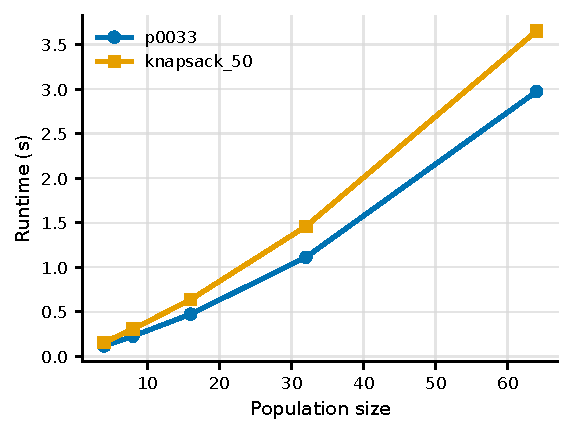
\includegraphics[width=\textwidth]{figures/sensitivity_population_size_nature.pdf}
    \caption{Population size}
\end{subfigure}
\caption{Representative sensitivity trends from the corrected 390-run study. The method exhibits a broad practical plateau rather than a narrow hyperparameter optimum, which is encouraging for low-tuning deployment.}
\label{fig:sensitivity}
\end{figure}

It is also worth clarifying what the sensitivity study does and does not show. Because it is run on the four audited feasibility-recovery instances, it is primarily a \emph{stability} analysis of the mainline implementation rather than a substitute for the official MIPLIB 2017 extension. The two studies therefore play different roles in the paper. The sensitivity analysis shows that the audited feasibility-recovery result is not brittle; the official extension shows how far the same mechanism generalizes once the benchmark becomes materially harder.

\subsection{Discussion}
\label{subsec:discussion}

Taken together, the experiments support a precise interpretation of the method. HP-PDHG is already convincing as a \emph{feasibility-recovery heuristic} on audited instances where the LP relaxation points toward a good basin but the final integrality transition remains difficult. The four-instance benchmark, the 20-seed robustness study, the p0282 trade-off plots, and the ablation study all point to the same mechanism: staged movement from relaxation quality to strict feasibility.

From a practical standpoint, many decision-support workflows cannot act on an infeasible solution, even when its objective looks attractive. In deadline-constrained planning settings, the key question is often whether the solver can supply a valid incumbent before the decision window closes. The p0282 trade-off plot therefore illustrates a realistic operational choice: accepting a slightly weaker objective in exchange for a deployable plan.

The larger official benchmark and the population-based baseline study refine that claim rather than overturn it. On the official 12-instance subset, the current implementation still does not deliver broad strict feasibility under a fixed 1000-iteration budget, but it does reduce audited violation on eight instances and wins the paired official-benchmark Wilcoxon test. On the representative six-instance metaheuristic comparison, the proposed method achieves the best average Friedman rank and the overall Friedman test is significant, but the Holm-adjusted post-hoc tests remain conservative. These findings are scientifically useful because they draw a credible boundary around the contribution. The present solver is stronger at structured feasibility-oriented search than at universal large-scale dominance. That is a narrower claim than ``this method beats all MIP heuristics,'' but it is also a claim that the audited evidence actually supports.

This boundary suggests a practical deployment strategy. HP-PDHG is best interpreted not as a replacement for mature exact solvers, but as a modular incumbent-generation or feasibility-restoration component within a broader optimization pipeline. It can warm-start branch-and-bound, serve as an anytime recovery layer, or provide a feasibility-first front end when decision validity is more urgent than proof of optimality. Because its modules are explicit, the framework is also amenable to policy control, learned scheduling, and domain-specific customization.
